\selectlanguage{italian}

I sistemi macroscopici realizzano l'equilibrio termodinamico bilanciando la tendenza dell'energia interna a diminuire e quella dell'entropia ad aumentare: ad alte temperature prevale il contributo entropico, a basse temperature prevale quello energetico (nei solidi gli atomi hanno posizioni fisse, dunque l'entropia è più basse rispetto ai fluidi). Sperimentalmente, infatti, si trova che quasi tutti i materiali solidificano a temperature abbastanza basse: l'unica eccezione è l'elio, che rimane fluido fino a $ T \approx 0 \,\text{K} $, a meno che non si applichi una sufficiente pressione. \\
Così come la tendenza degli atomi a formare molecole (minimizzando $ V_\text{ad} $) viene misurata dalla binding energy molecolare, la tendenza di atomi/molecole a formare solidi viene misurata da una quantità analoga, l'\textit{energia di coesione}.

\section{Struttura microscopica}

Nello studio di solidi semplici, come ad esempio quelli formati da gas nobili, l'interazione tra atomi è semplificabile a coppie, quindi modellizzabile con il potenziale di Lennard-Jones:
\begin{equation}
	V_\text{ad}(\ve{R}_1 , \dots , \ve{R}_{N_n}) = \sum_{\alpha < \alpha'}^{N_n} V_2(\abs{\ve{R}_\alpha - \ve{R}_{\alpha'}})
	\qquad \qquad
	V_2(r) = 4\varepsilon \left[ \left( \frac{\sigma}{r} \right)^{12} - \left( \frac{\sigma}{r} \right)^6 \right]
\end{equation}
Per un coppia di atomi, la distanza d'equilibrio è $ R_\text{m} = \sqrt[6]{2} \sigma $ con potenziale minimo $ V_2(R_\text{m}) = -\varepsilon $. Inoltre, si vede che il potenziale decade come $ \sim r^{-6} $, quindi, contando che tipicamente il numero di atomi a distanza $ r $ da un dato atomo scala come $ \sim r^2 $, l'energia d'interazione totale a lunga distanza scala come $ r^{-4} $: si vede che ogni atomo interagisce significativamente soltanto con gli atomi ad esso vicini. \\
Si consideri un reticolo 1D di atomi: aggiungendo un terzo atomo ad una coppia di atomi, esso si posizionerà ad una distanza $ \approx R_\text{m} $ da essi (ignorando l'interazione tra secondi-vicini) ed abbasserà la buca di potenziale adiabatico a $ \approx -2\varepsilon $. Ciò è generalizzabile ad $ N_n $ atomi: essi si troveranno a distanza $ \approx R_\text{m} $ l'uno dall'altro e l'energia di coesione totale sarà $ \approx (N_n - 1) \varepsilon $ (circa $ \varepsilon $ per atomo, per $ N_n $ grande). Se si considera l'interazione con secondi- e terzi-vicini, si trova che la distanza d'equilibrio è leggermente minore rispetto a $ R_\text{m} $ e che l'energia di coesione è leggermente maggiore di $ (N_n - 1) \varepsilon $ (si veda Fig. \ref{lat-2}a). \\
Se invece si considera un reticolo 2D, il terzo atomo si posizionerà al vertice di un triangolo equilatero formato con i primi due. Aggiungendo altri atomi, si viene a formare un \textit{reticolo triangolare} (o esagonale, si veda Fig. \ref{lat-2}), in cui ciascun atomo a 6 primi-vicini, dunque l'energia di coesione sarà approssimativamente $ 3\varepsilon $ per atomo (6 legami condivisi da 2 atomi ciascuno). Si vede dunque che il modello d'interazione a coppie porta al principio di \textit{massima coordinazione}: gli atomi si dispongono in modo da massimizzare il numero di primi-vicini, così da massimizzare l'energia di coesione (minimizzando l'energia potenziale adiabatica). \\
Applicando il principio di massima coordinazione ad un reticolo 3D, si vede che 4 atomi massimizzano la loro coordinazione ponendosi ai vertici di un tetraedro regolare: gli atomi successivi si dispongono a formare o il \textit{face-centered cubic lattice} (reticolo fcc, Fig. \ref{lat-3}b) o l'\textit{hexagonal close-packed lattice} (reticolo hcp, Fig. \ref{lat-3}c). In entrambi questi reticoli ogni atomo ha 12 primi-vicini, dunque l'energia reticolare è $ 6\varepsilon $ per atomo; si vede, però, che entrambi sono formati da reticoli triangolari 2D sovrapposti: mentre nell'fcc si ripetono 3 orientazioni diverse, nell'hcp ce ne sono solo 2, dunque, quando si va a considerare l'interazione con secondi- e terzi-vicini, il reticolo fcc è leggermente favorito energeticamente rispetto all'hcp. \\
Confrontando i vari reticoli, si trovano delle distanze d'equilibrio leggermente diverse: in 1D $ R_\text{m} = \sqrt[6]{2} \sigma \simeq 1.22 \sigma $, in 2D $ R_\text{m} \simeq 1.11 \sigma $ ed in 3D $ R_\text{m} \simeq 1.09 \sigma $. Nella tavola periodica c'è una prevalenza a formare cristalli fcc ed hcp: ci sono alcuni bcc (body-centered cubic, simile all'fcc ma con un atomo al centro del cubo, al posto di quelli sulle facce) ed i casi del diamante (struttura a sé) e del polonio, che invece forma l'sc (simple cube). \\
È possibile formare strutture cristalline\footnote{Si noti che i vetri, al contrario dei cristalli, hanno una risposta plastica alle deformazioni: essi non sono solidi, ma liquidi con coefficiente di viscosità estremamente elevato, caratterizzati da livelli energetici estremamente vicini. Infatti, osservando i vedtri di edifici antichi, essi risulteranno ondulati, in quanto deformati nel tempo dalla gravità.} diverse da quelle descritte considerando un potenziale non necessariamente a 2 corpi (valido principalmente per gas nobili, che hanno interazioni deboli): potenziali a più corpi introducono effetti elettronici (quantistici) che danno direzionalità ai legami, fino ad arrivare ai solidi con legami metallici covalenti in cui le interazioni si estendono alla totalità del solido, impedendo di fattorizzare la funzione d'onda.

\begin{figure}[!h]
	\centering
	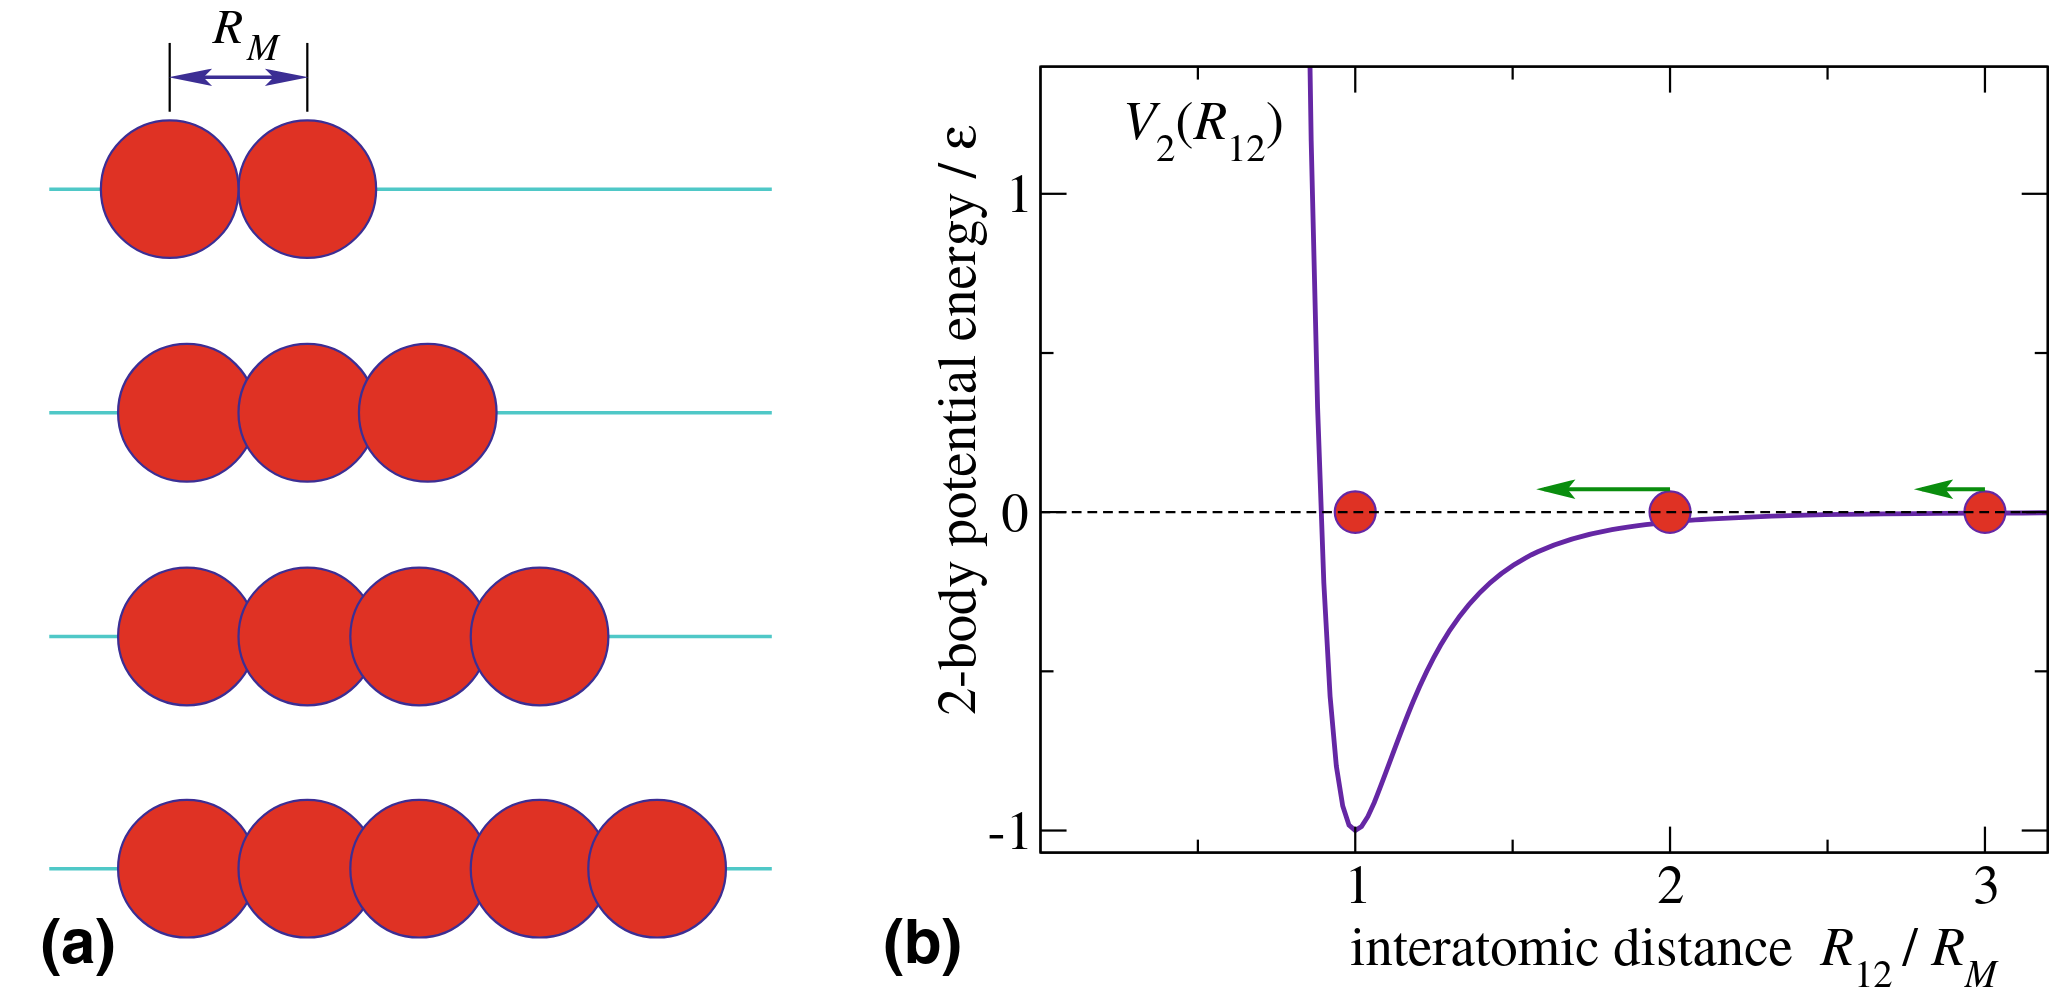
\includegraphics[width = 0.45 \textwidth]{lattice-1d.png}
	\qquad
	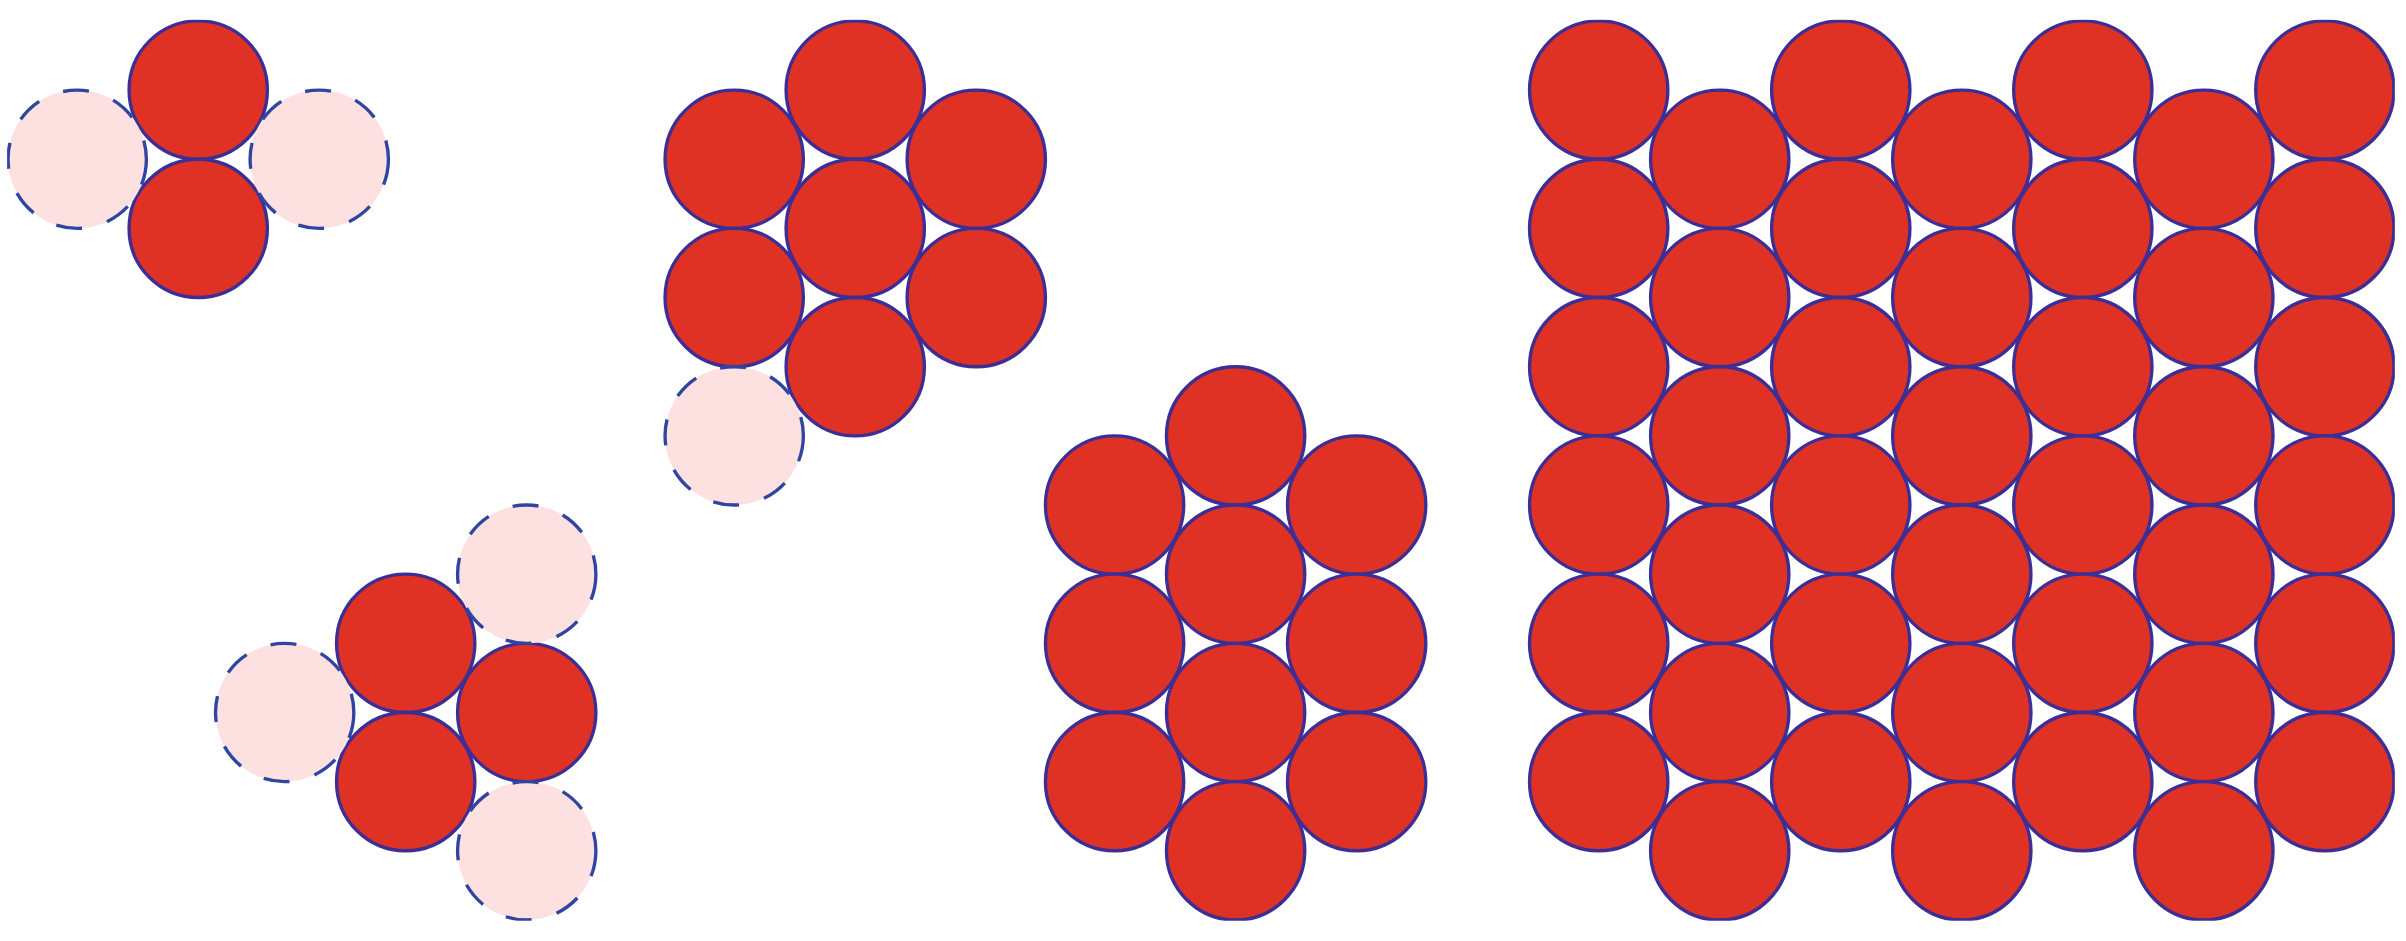
\includegraphics[width = 0.45 \textwidth]{lattice-2d.png}
	\caption{1D lattice and 2D triangular lattice of atoms.}
	\label{lat-2}
\end{figure}
\begin{figure}[!h]
	\centering
	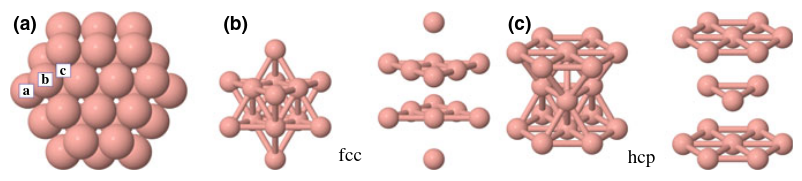
\includegraphics[width = 0.70 \textwidth]{lattice-3d.png}
	\caption{3D lattices of atoms: (a) close packing of spheres, (b) fcc lattice, (c) hcp lattice.}
	\label{lat-3}
\end{figure}

\paragraph{Difetti}

Un cristallo, a qualunque temperatura finita, ha probabilità non-nulla di formare dei \textit{difetti}, come ad esempio un atomo mancante, un atomo aggiuntivo o un'impurità (atomo di tipo diverso). In particolare, essendo il numero di atomi in un cristallo estremamente grande, la concentrazione dei difetti in un cristallo all'equilibrio a bassa temperatura va come $ \sim e^{- \beta E} $ (statistica di Boltzmann), dove $ E \sim 1 \ev $ è l'energia tipica di formazione di un difetto. Termodinamicamente, è impossibile creare un cristallo con un'estensione finita privo di difetti. \\
La piccola differenza energetica tra reticoli fcc ed hcp permette la formazione di difetti estesi (al limite anche macroscopici) come dislocazioni, stacking faults e bordi di grano (vedere Figg. \ref{def-disl}-\ref{def-st-gr}). Una dislocazione avvience quando un layer a cui manca un atomo si collega ad un layer completo: queste configurazioni sono metastabili, e con un'energia finita, a temperatura sufficientemente elevata, è possibile spostare questi difetti all'interno del cristallo. Una stacking fault avviene invece quando si interrompe e viene modificata l'alternanza regolare dei layer, mentre un bordo di grano si verifica quando si sviluppa un cristallo a partire da due punti di duplicazione diversi e con orientazioni diverse, andando a creare un'interfaccia disordinata quando queste orientazioni si incontrano.

\begin{figure}[!h]
	\centering
	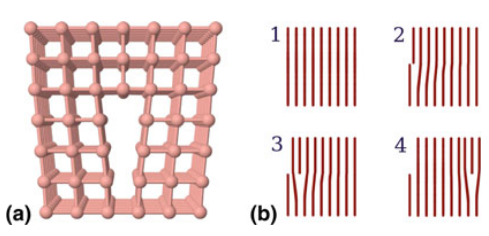
\includegraphics[width = 0.50 \textwidth]{def-disl.png}
	\caption{Dislocation in an sc lattice.}
	\label{def-disl}
\end{figure}
\begin{figure}[!h]
	\centering
	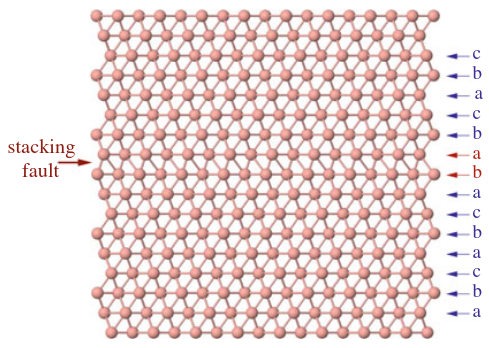
\includegraphics[width = 0.40 \textwidth]{def-st.png}
	\qquad \qquad
	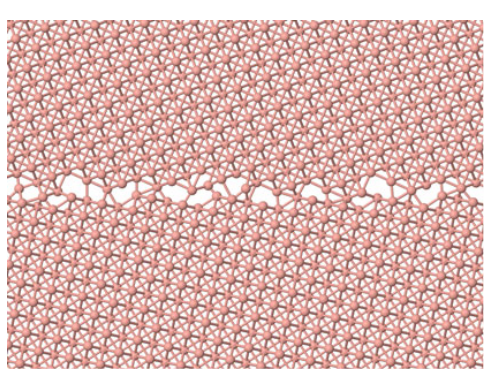
\includegraphics[width = 0.40 \textwidth]{def-gr.png}
	\caption{Stacking fault and grain boundary in an fcc lattice.}
	\label{def-st-gr}
\end{figure}

\subsection{Reticoli cristallini}

Una delle proprietà fondamentali di un solido cristallino è l'equivalenza di varie sue regioni di spazio: infatti, si può assumere che la maggior parte degli atomi di un cristallo si trovino sufficientemente lontani dal suo bordo e da qualsiasi difetto per essere modellato come appartenente ad un cristallo perfetto ed infinitamente esteso. \\
Un cristallo perfetto infinito è un insieme di punti che gode di simmetria traslazionale discreta.

\begin{definition}{Reticolo di Bravais}{}
	Si dice \textit{reticolo di Bravais} $ n $-dimensionale un insieme di punti in $ \R^n $ che risulta invariante per traslazioni discrete:
	\begin{equation}
		\ve{r} \mapsto \ve{r}' = \ve{r} + \ve{R}
		\ , \
		\ve{R} = k_1 \ve{a}_1 + \dots k_n \ve{a}_n
	\end{equation}
	con $ \{k_j\}_{j = 1,\dots,n} \subset \Z $ e $ \{\ve{a}_j\}_{j = 1,\dots,n} \subset \R^n $ linearmente indipendenti.
\end{definition}

I generatori $ \{\ve{a}_j\}_{j = 1,\dots,n} $ vengono detti \textit{primitivi} se sono $ \virgolette{i più piccoli possibili} $ (non univocamente definiti) e formano una cella primitiva, ovverosia il volume minimo che contiene tutti i punti traslazionalmente non-equivalenti del reticolo (a meno di traslazioni) e che, ripetuto nello spazio tramite traslazioni discrete, riproduce il reticolo. Nel caso tridimensionale, il volume della cella primitiva è $ V_c = \abs{(\ve{a}_1 \cdot \ve{a}_2) \times \ve{a}_3} $. \\
La cella primitiva contiene tutta l'informazione del reticolo (che è una ripetizione di tale cella), dunque il suo studio è fondamentale. Il problema, nel definirla, è che non c'è un univoco set di vettori primitivi.

\begin{definition}{Cella di Wigner-Seitz}{}
	Dato punto $ \ve{R} $ in un reticolo di Bravais, si definisce la \textit{cella di Wigner-Seitz} l'insieme di punti $ \ve{r} $ più vicini ad $ \ve{R} $ rispetto ad un altro punto $ \ve{R}' $ del reticolo.
\end{definition}

\begin{proposition}{}
	La cella di Wigner-Seitz è una cella primitiva.
\end{proposition}

L'introduzione della cella di Wigner-Seitz elimina l'arbitrarietà nella scelta della cella primitiva.

\begin{figure}
	\centering
	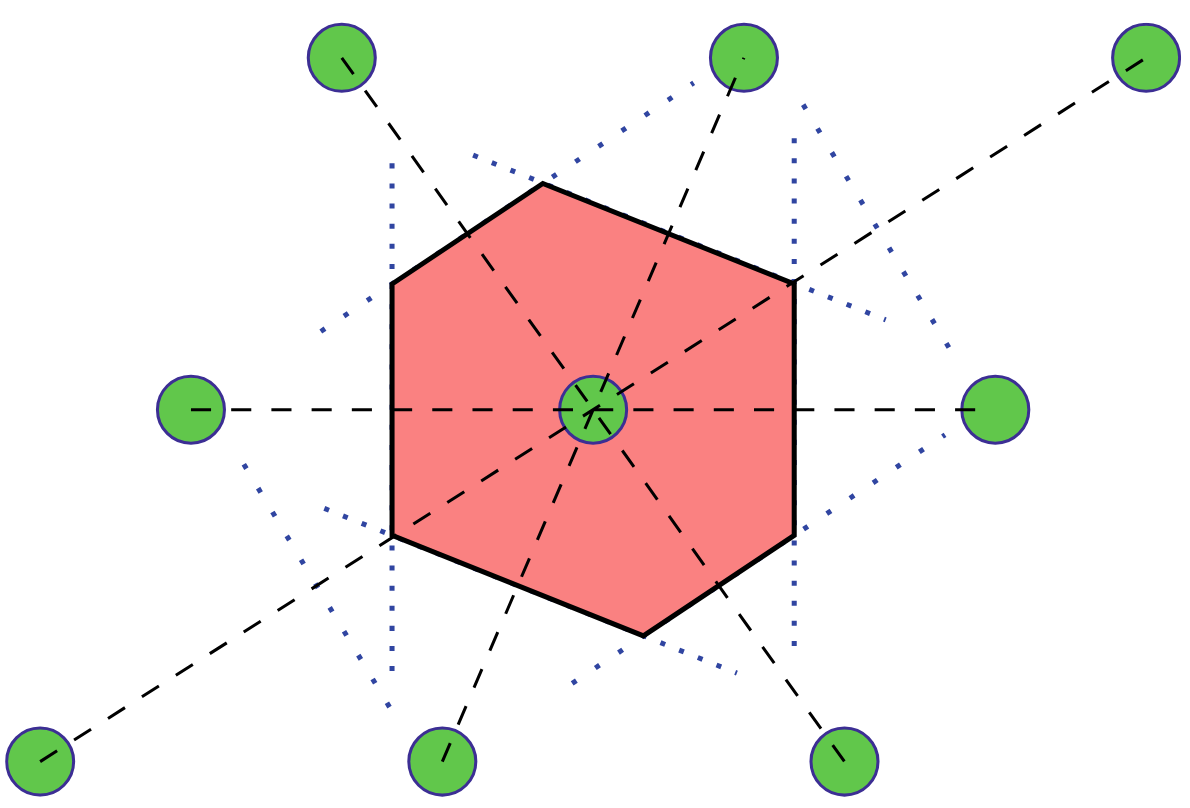
\includegraphics[width = 0.50 \textwidth]{ws-2.png}
	\caption{Wigner-Seitx cell for a 2D lattice.}
	\label{ws-2}
\end{figure}
\begin{figure}
	\centering
	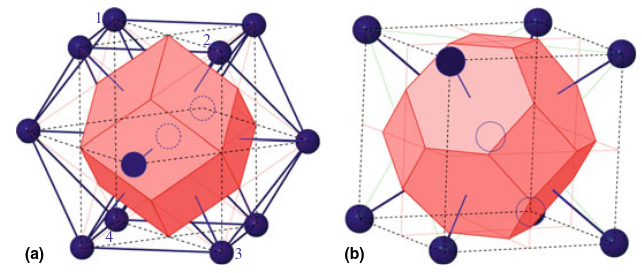
\includegraphics[width = 0.50 \textwidth]{ws-3.png}
	\quad
	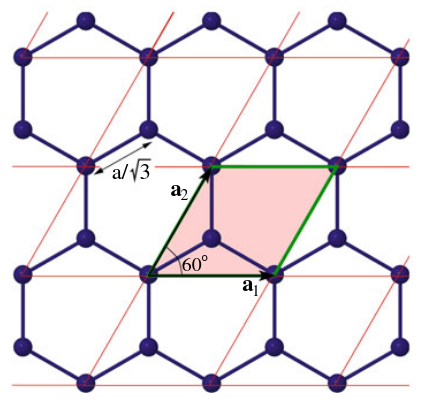
\includegraphics[width = 0.30 \textwidth]{ws-g.png}
	\caption{Wigner-Seitx cell for the fcc lattice, the bcc lattic and graphene.}
	\label{ws-3}
\end{figure}

Si noti che, in generale, una cella primitiva può contenere più di un atomo (es.: $ \ch{Na Cl} $, grafite, etc.). Infatti, un cristallo è definito da un reticolo di Bravais e da una base, ovvero un insieme di uno o più atomi ripetuti in ogni punto del retivolo. È inoltre conveniente trattare le cosiddette \textit{celle convenzionali}, ovvero insiemi di una o più celle primitive che hanno forme preferibilmente cubiche (fcc, bcc o sc), per facilitare la trattazione. Bisogna tener conto che le celle convenzionali, essendo delle super-celle, contengono informazioni ridondanti rispetto alle celle primitive.

\subsubsection{Reticolo reciproco}

Si consideri una funzione $ f : \R \rightarrow \R $ periodica con periodo $ a \in \R $, ovvero tale per cui $ f(x -na) = f(x) \,\,\forall n \in \Z $. La sua antitrasformata di Fourier è:
\begin{equation}
	f(x) = \int_\R \frac{\dd k}{\sqrt{2\pi}} e^{ikx} \tilde{f}(k)
\end{equation}
I coefficienti di Fourier $ \tilde{f}(k) $ sono nulli, eccetto quelli con lo stesso periodo di $ f(x) $, ovvero quelli con $ e^{ikx} = e^{ik(x-a)} $: ciò equivale a $ e^{-ika} = 1 $, ovvero $ k = \ell \frac{2\pi}{a} $, con $ \ell \in \Z $. Questi valori vengono convenzionalmente indicati come:
\begin{equation}
	G = \frac{2\pi}{a} \ell
\end{equation}
e forniscono le frequenze discrete, nello spazio reciproco, che costituiscono la serie di Fourier di $ f(x) $:
\begin{equation}
	f(x) = \sum_G e^{iGx} \tilde{f}(G)
	\qquad \qquad
	\tilde{f}(G) = \frac{1}{a} \int_0^a \dd x\, e^{-i G x} f(x)
\end{equation}
I punti $ G $ nello spazio reciproco formano un reticolo, detto \textit{reticolo reciproco}, legato al reticolo nello spazio diretto da:
\begin{equation}
	e^{i G R} = e^{i 2\pi n \ell} = 1
\end{equation}
dove $ R = na $ sono le traslazioni del reticolo diretto. Si trova quindi $ \ell = \frac{1}{n} $. \\
Queste definizioni sono generalizzabili al caso 3D, in cui $ \ve{R} = n_1 \ve{a}_1 + n_2 \ve{a}_2 + n_3 \ve{a}_3 $. In questo caso, la condizione di reciprocità diventa:
\begin{equation}
	e^{i \ve{G} \cdot \ve{R}} = 1
\end{equation}
In 3D si trova che:
\begin{equation}
	\ve{G} = \ell_1 \ve{b}_1 + \ell_2 \ve{b}_2 + \ell_3 \ve{b}_3
\end{equation}
con $ \ell_1, \ell_2, \ell_3 \in \Z $ e:
\begin{equation}
	\ve{b}_1 = \frac{2\pi}{V_c} \ve{a}_2 \times \ve{a}_3
	\qquad
	\ve{b}_1 = \frac{2\pi}{V_c} \ve{a}_2 \times \ve{a}_3
	\qquad
	\ve{b}_1 = \frac{2\pi}{V_c} \ve{a}_2 \times \ve{a}_3
\end{equation}
Si noti che $ \ve{a}_i \cdot \ve{b}_j = 2\pi $, dunque $ \ve{G} \cdot \ve{R} = 2\pi (n_1 \ell_1 + n_2 \ell_2 + n_3 \ell_3) $. La serie di Fourier in 3D diventa:
\begin{equation}
	f(\ve{x}) = \sum_\ve{G} e^{i \ve{G} \cdot \ve{x}} \tilde{f}(\ve{G})
	\qquad \qquad
	\tilde{f}(\ve{G}) = \frac{1}{V_c} \int_{V_c} \dd^3x\, e^{-i \ve{G} \cdot \ve{x}} f(\ve{x})
\end{equation}
Il volume della cella primitiva del reticolo reciproco è $ \tilde{V}_c = (\ve{b}_1 \times \ve{b}_2) \cdot \ve{b}_3 = \frac{(2\pi)^3}{V_c} $: questa viene detta \textit{prima zona di Brillouin} (BZ).

\begin{example}{Reticoli reciproci}{}
	Il reticolo reciproco di un fcc con cubo di lato $ a $ è un bcc con cubo di lato $ 4\pi/a $ e viceversa, mentre il reticolo reciproco di un sc con cubo di lato $ a $ è un sc con cubo di lato $ 2\pi/a $.
\end{example}

Ciascun $ \ve{G} $ nel reticolo reciproco definisce un'onda piana $ e^{i \ve{G} \cdot \ve{x}} $ (nello spazio diretto) con la stessa periodicità del reticolo diretto. Se si considerano i fronti d'onda fissati, per esempio, da $ e^{i \ve{G} \cdot \ve{x}} = 1 $, questi formano una famiglia di piani paralleli tra loro e perpendicolari a $ \ve{G} $ (che ne dà la direzione di propagazione), separati tra loro da una distanza $ \lambda = 2\pi / \abs{\ve{G}} $. \\
Alcuni di questi piani passano per punti del reticolo reciproco; in particolare, tutti questi piani passano per punti del reticolo reciproco se gli indici interi $ (\ell_1 \, \ell_2 \, \ell_3) $ che definiscono $ \ve{G} $ non hanno divisori non-banali comuni: questi vengono detti \textit{indici di Miller} della famiglia di piani considerata. Se invece $ \ve{G} $ è determinato da $ (n\ell_1 \, n\ell_2 \, n\ell_3) $, con $ n \in \Z - \{0\} $, allora soltanto un piano ogni $ n $ passerà per punti del reticolo diretto. \\
Si dimostra che gli indici di Miller sono proporzionali ai reciproci delle intercette dei piani con le direzioni dei vettori primitivi del reticolo diretto.








